\documentclass{article}
\usepackage{geometry}
\geometry{a4paper, top=3cm, bottom=3cm, left=2cm, right=2cm}
\usepackage[utf8]{inputenc}
\usepackage[english]{babel}
\usepackage{hyperref}
\makeindex

\title{OpenGL exercises}
\author{Riccardo Salvalaggio}
\date{17th of May, 2021}

\usepackage{amssymb}
\usepackage{amsmath}
\usepackage{txfonts}
\usepackage{mathdots}
\usepackage[classicReIm]{kpfonts}
\usepackage{graphicx}
\usepackage{listings}
%\usemintedstyle{borland}
\begin{document}

\maketitle
\newpage
\tableofcontents
\newpage

\section{Introduction}
The \textbf{OpenGL Extension Wrangler (GLEW)} is what we will be using to give us access to the OpenGL 3.2 API functions.  In modern OpenGL, the API functions are determined at run time, not compile time.\\\\
\textbf{GLFW} will allow us to create a window, and receive mouse and keyboard input in a cross-platform way.\\\\
\textbf{OpenGL Mathematics (GLM)} is a mathematics library that handles vectors and matrices, amongst other things.\\\\
\textbf{Shaders: }Shaders are little programs, made from GLSL code, that run on the GPU instead of the CPU. In older version of OpenGL, shaders were optional. In modern OpenGL, shaders are required. What they do depends on types.\\\\
\textbf{- Types of shaders: }\\
\textbf{1. Vertex shaders: }transform points.\\\\
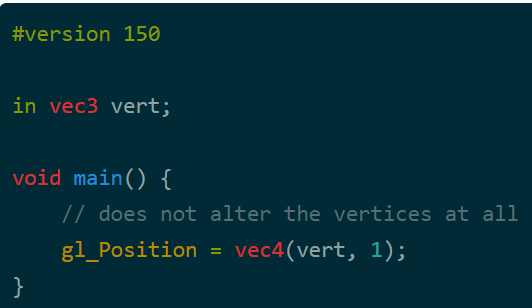
\includegraphics[scale=0.6]{1.png}\\\\
First shader: in vec3 vert is just a 3d vetex, gl$\_$position is needed in every shader, in this case just transform the 3d vertex in a 4d one without modifying anything.\\
\textbf{2. Fragment shaders: }  calculate the color of each pixel that is drawn. A “fragment” is basically a pixel, so you can think of fragment shaders as “pixel shaders.”  
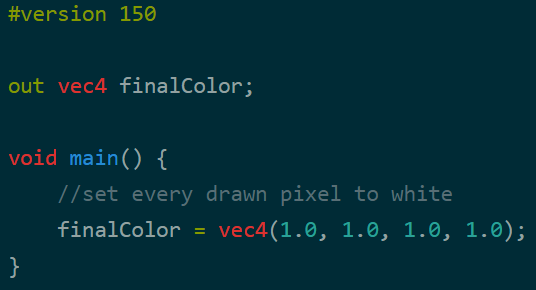
\includegraphics[scale=0.6]{2.png}\\\\
First fragment shader: deine output colored variable, vec4(R,G,B,$\alpha$).\\\\

\subsection{VBO and VAO}
Vertex Buffer Objects (VBOs) and Vertex Array Objects (VAOs) are used to take data from your C++ program and send it through to the shaders for rendering (exchnge data between CPU and GPU). \\
VBOs are "buffers" of video memory – just a bunch of bytes containing any kind of binary data you want.\\
VAOs are the link between the VBOs and the shader variables. VAOs describe what type of data is contained within a VBO, and which shader variables the data should be sent to.
\begin{quote}
In this article, we will use a VAO to say “hey OpenGL, this VBO right here has 3D points in it, and I want you to send those points to the ‘vert’ variable in the vertex shader.”
\end{quote}

\section{Exercise 1}
First initialise GLFW for error handler, then to create window \textit{glfwwindowshint}, \textit{glfwCreateWindow} and \textit{glfwMakeContextCurrent(gWindow);}.\\
Now we have the windows, we initialise GLEW to access API.\\
Inside the LoadShaders function, we compile and link a vertex shader and a fragment shader. Inside the LoadTriangle function, we are going to make one VBO and one VAO. Next, we upload some data into the new VBO. It is time to set up the VAO. First, we are going to enable the vert variable in the shader program. The most complicated part of VAO setup is this next function: glVertexAttribPointer:\\
\begin{quote}
glVertexAttribPointer(gProgram$->$attrib("vert"), 3, GL$\_$FLOAT, GL$\_$FALSE, 0, NULL);
\end{quote} 
Now that the VBO and VAO are fully set up, we unbind them so they don’t accidentally get used somewhere else. 
At this point, the shaders, VBO, and VAO are ready for use. All we have to do now is draw them inside the Render function.\\
First we clear the screen so that it is completely black:
\begin{quote}
glClearColor(0, 0, 0, 1); // black\\
glClear(GL$\_$COLOR$\_$BUFFER$\_$BIT | GL$\_$DEPTH$\_$BUFFER$\_$BIT);
\end{quote}
Next we tell OpenGL that we want to start using our shaders and our VAO:
\begin{quote}
glUseProgram(gProgram->object());\\
glBindVertexArray(gVAO);
\end{quote}
At last, we can draw that ever-elusive triangle:
\begin{quote}
glDrawArrays(GL$\_$TRIANGLES, 0, 3);
\end{quote}
This call to glDrawArrays says that we want to draw triangles, starting at vertex zero, and ending after three vertices have been sent to the shader. It will look at the currently bound VAO to determine where to get the vertices from. The vertices will be pulled out of the VBO and sent to the vertex shader. The drawing is finished now, so we unbind the shaders and the VAO just to be safe\\ 
The last thing that needs to be done before we can see the triangle is to swap the frame buffers:
\begin{quote}
glfwSwapBuffers(gWindow);
\end{quote}
Before the frame buffers were swapped, we were drawing to an off-screen frame buffer that was not visible in the window we created at the start.

\section{Exercise 2}

\includegraphics[scale=0.6]{3.png}\\\\
We will be adding a texture to the triangle.

\subsection{Uniform vs Attribute Shader Variables}
Attribute variables can have a different value for each vertex. Uniform variables keep the same value for multiple vertices. Uniforms can be accessed from any shader, but attributes must enter the vertex shader first, not the fragment shader. The vertex shader can pass the value into the fragment shader if necessary. To set the value of a uniform, we use one of the glUniform* functions. To set the value of an attribute, we store the values in a VBO and send them to the shader with a VAO and glVertexAttribPointer. It is also possible to set the value of an attribute using one of the glVertexAttrib* functions, if you are not storing the values in a VBO.\\
\subsection{Textures}
Textures are basically 2D images that you can apply to your 3D objects.  That is, you upload the data for the texture to the graphics card before you can use it. This is similar to how we saw VBOs working in the previous article – VBOs are used to store data in video memory before that data gets used.\\\\
We will use the tdogl::Bitmap class to load the raw pixel data from “hazard.png” into memory, with the help of stb$\_$image. Then we will use tdogl::Texture to upload the raw pixel data into an OpenGL texture object.\\
\subsection{Texture coordinates}
Coordinates are not in pixels. They range from zero to one, where (0,0) is the bottom left and (1,1) is the top right.
\subsection{Texture Image Units}
You can't just send a texture straight to a shader. First you bind the texture to a texture unit, then you send the index of the texture unit to the shader. We will only be using one texture in this article, so we only need one texture unit. 
\subsection{Implementing Textures}
First we define a global variable for the Texture. Then get the texture:\\
\begin{quote}
static void LoadTexture() {
    tdogl::Bitmap bmp= tdogl::Bitmap::bitmapFromFile(ResourcePath("hazard.png"));
    bmp.flipVertically(	);
    gTexture = new tdogl::Texture(bmp);
}	
\end{quote}
Next we will give each vertex of the triangle a texture coordinate. We can’t pass an attribute straight into the fragment shader, because attributes must first go through the vertex shader. Here is the modified vertex shader:\\
\begin{quote}
#version 150
in vec3 vert;
in vec2 vertTexCoord;
out vec2 fragTexCoord;

void main() {
    // Pass the tex coord straight through to the fragment shader
    fragTexCoord = vertTexCoord;
    
    gl_Position = vec4(vert, 1);
}
\end{quote}




\end{document}